\subsection{Etherless-smart}

\subsubsection{Struttura}
  Il compito del modulo Etherless-smart è di:
  \begin{itemize}
    \item gestire la comunicazione tra gli altri due moduli che compongono il prodotto;
    \item gestire il pagamento per le operazioni eseguite dagli utenti sulla piattaforma \textit{Etherless}.
  \end{itemize}
  Per implementare queste funzionalità abbiamo sviluppato i seguenti smart contract:
  \begin{itemize}
    \item \textbf{EtherlessSmart:} gestisce la comunicazione con con gli altri due moduli mediante la definizione di metodi pubblici ed emette eventi sulla rete Ethereum. Comunica inoltre con i contratti EtherlessEscrow ed EtherlessStorage per gestire le operazioni di pagamento e di lettura e scrittura dei dati relativi alle funzioni;
    \item \textbf{EtherlessStorage:} gestisce la memorizzazione e la lettura dei dati delle funzioni eseguibili dall'utente (di cui è stato quindi fatto il deploy su AWS-Lambda) sulla rete Ethereum;
    \item \textbf{EtherlessEscrow:} contiene tutti gli estremi delle transazioni in corso e permette la gestione dei pagamenti in modalità escrow, con eventuale rimborso all'utente in caso se ne presenti la necessità.
  \end{itemize}

\subsubsection{Design}
  Il modulo Etherless-smart è stato progettato con lo scopo di ridurre il costo delle transazioni, eliminandolo dove possibile per le operazioni che richiedono la sola lettura dei dati. A questo scopo tutte le funzioni che non modificano la memoria interna del contratto sono contrassegnate dal modificatore \texttt{view}, indicando al compilatore che il metodo è in sola lettura e non in scrittura. \\
  Per quanto concerne i design pattern invece, essendo \textit{Solidity} diverso dai paradigmi di programmazione ad oggetti, abbiamo individuato dei design pattern e delle \textit{best practices} proprie del linguaggio, che abbiamo poi usato durante la fase di progettazione. In particolare, i design pattern a cui abbiamo fatto riferimento sono:
  \begin{itemize}
    \item \textbf{Access Restriction:} alcuni metodi messi a disposizione nel modulo Etherless-smart sono contrassegnati come pubblici in quanto vengono chiamati dall'esterno del contratto stesso (da un altro contratto o dai moduli CLI e Server). Tuttavia, ciò implica la possibilità per questi metodi di essere invocati da chiunque interagisca con la Blockchain Ethereum. Per motivi di sicurezza, l'accesso ad alcune funzioni viene limitato ad indirizzi specifici nei seguenti modi:
      \begin{itemize}
        \item \textbf{derivazione dal contratto \texttt{Ownable}:} le funzioni di pagamento del contratto EtherlessEscrow devono essere disponibili solo per il contratto EtherlessSmart; è possibile ottenere questa restrizione derivando EtherlessEscrow dal contratto \texttt{Ownable} fornito da \textit{OpenZeppelin}: in questo modo tutti i metodi di EtherlessEscrow contrassegnati dal modificatore \texttt{onlyOwner} saranno invocabili solo dall'indirizzo che ha provveduto all'istanziazione del dato contratto, che nel nostro caso è EtherlessSmart;
        \item \textbf{modificatori d'accesso:} le funzioni di risposta (come \texttt{runResult}, \texttt{deployResult}, etc.) devono poter essere chiamate solo da Etherless-server; riusciamo ad ottenere ciò implementando in EtherlessSmart un modificatore apposito \texttt{onlyServer}, che permetterà l'invocazione dei metodi contrassegnati come tali solo dall'indirizzo corrispondente.
      \end{itemize}

    \item \textbf{Secure Ether Transfer:} il trasferimento di ETH da un indirizzo ad un'altro è gestito in modo sicuro dal contratto EtherlessEscrow, che nelle funzioni di trasferimento dei fondi utilizza il metodo \texttt{sendValue}, fornito dal contratto \texttt{Address} offerto da \textit{OpenZeppelin}. Inoltre, la divisione dal contratto EtherlessSmart dei metodi che gestiscono il pagamento protegge da eventuali attacchi che potrebbero impossessarsi di denaro.

    \item \textbf{String Equality Comparison:} allo stato attuale Solidity non offre funzionalità di comparazione tra stringhe, quindi abbiamo costruito un metodo apposito \texttt{compareString} che si occupa di verificare l'uguaglianza tra due stringhe. Per rendere questa operazione meno costosa in termini di gas, abbiamo seguito il pattern String Equality Comparison, che comporta, oltre al confronto per carattere, un previo confronto tra la lunghezza delle stringhe evitando controlli inutili e dispendiosi;

  \item \textbf{Proxy Delegate:} la blockchain Ethereum è immutabile, e, di conseguenza, una volta rilasciato un contratto questo non può più essere modificato. Tuttavia, una \textit{best practice} comunemente usata nell'ambito per ovviare a questo problema consiste nell'utilizzare un proxy che punta all'indirizzo dell'ultima versione del contratto rilasciata sulla rete, rendendo così i contratti aggiornabili. Si noti come i contratti precedenti non verranno sovrascritti, ma continueranno ad esistere nella rete: sembrerà tuttavia che sia avvenuto un aggiornamento del codice precedente perché il proxy provvederà a puntare all'ultimo contratto rilasciato. \\
    Il framework \textit{OpenZeppelin} fornisce una funzionalità di upgrade per gli smart contract che implementa il meccanismo di proxy forwarding dietro le quinte, semplificando la gestione dell'aggiornamento del codice dei contratti. \\
    I contratti EtherlessSmart ed EtherlessStorage sono stati implementati in modo da poter sfruttare questo meccanismo: ad una richiesta di upgrade di un contratto caricato sulla rete ad un certo indirizzo, \textit{OpenZeppelin} si occupa di "reindirizzarlo" in modo da mantenere lo stesso indirizzo sulla rete Ethereum riferendosi però all'implementazione aggiornata del contratto.
 \end{itemize}

\subsubsection{Diagramma delle classi}
Gli smart contract scritti in Solidity sono assimilabili alle classi dei linguaggi di programmazione ad oggetti, in quanto contengono attributi propri e metodi per effettuare operazioni su questi attributi. Per questo motivo abbiamo ritenuto adeguato usare i diagrammi delle classi con la sintassi UML per rappresentarne il contenuto. \\
Tuttavia, per l'ambito in cui viene utilizzato, Solidity presenta delle feature aggiuntive che non hanno nulla a che vedere con un paradigma di programmazione ad oggetti, come ad esempio il tipo di dato \texttt{address}, la possibilità di definire \texttt{payable} un metodo od un indirizzo, la definizione di specifici modificatori d'accesso e gli eventi. Per contrassegnare questi elementi mantenendo la sintassi UML abbiamo deciso di inserire l'informazione che li contraddistingue tra parentesi graffe alla fine della definizione dell'elemento. A ciò fanno eccezione gli indirizzi contrassegnati come \texttt{payable} che, essendo un tipo diverso dal semplice indirizzo, vengono indicati semplicemente come \texttt{address payable}.
\newgeometry{a4paper,left=1in,right=1in,top=1in,bottom=1in,nohead}
\begin{landscape}
  \begin{figure}[H]
    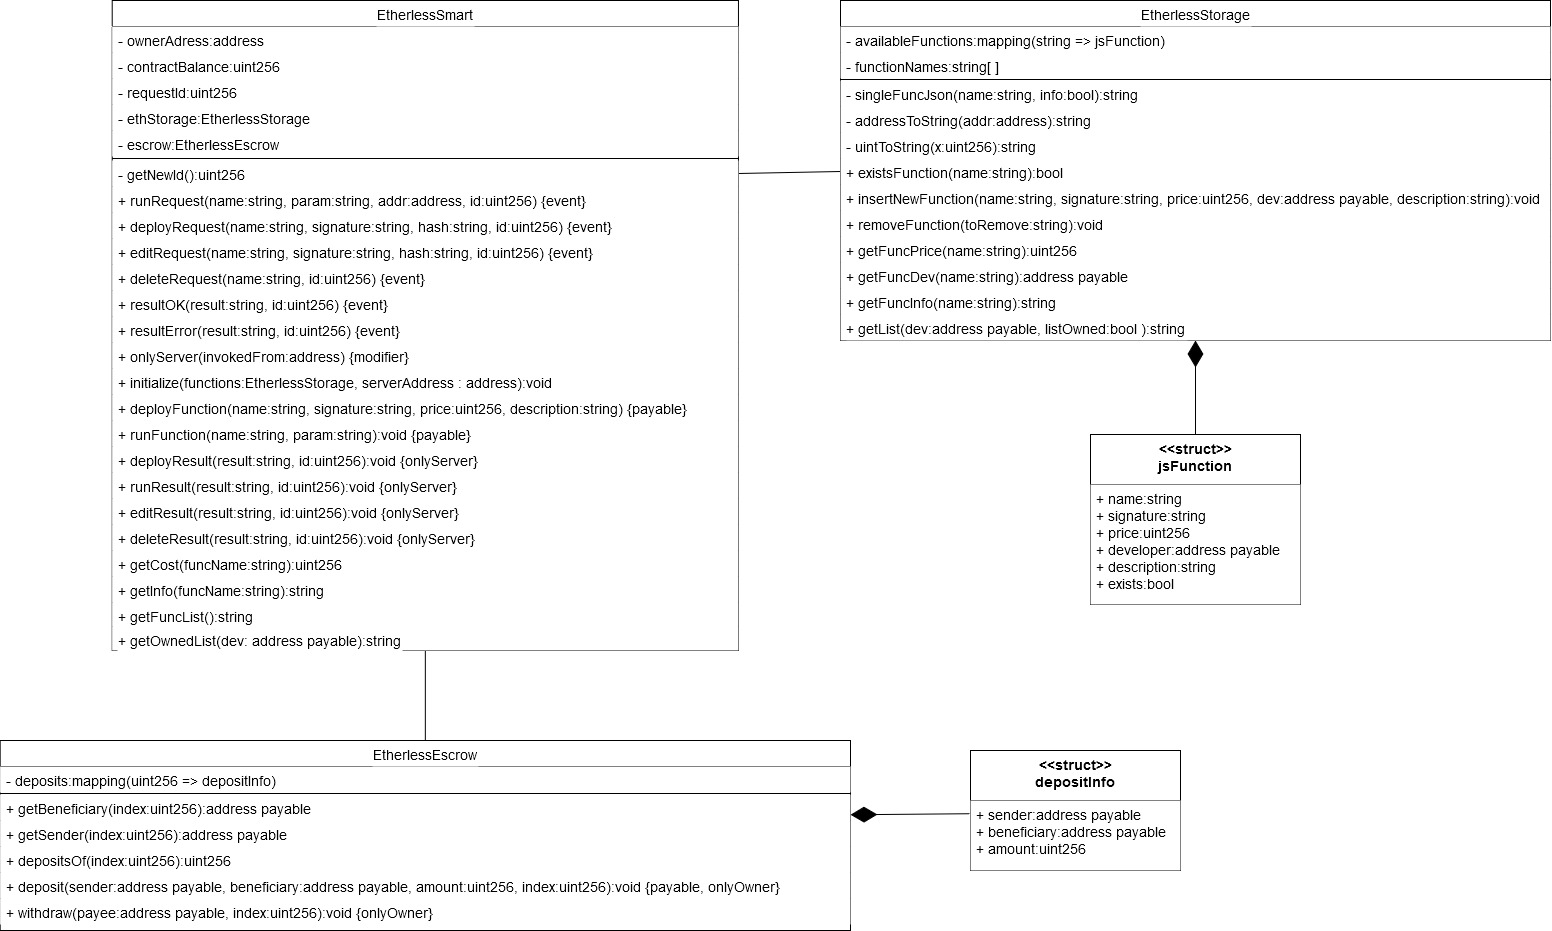
\includegraphics[width=21.5cm, height=14cm]{././diagrammi/etherless-smart/classi/Etherless-smart.jpg}
  	\caption{Diagramma delle classi Etherless-smart.}
  \end{figure}
\end{landscape}
\restoregeometry
\subsubsection{Diagrammi di sequenza}
\begin{figure}[H]
	\noindent
	\makebox[\textwidth]{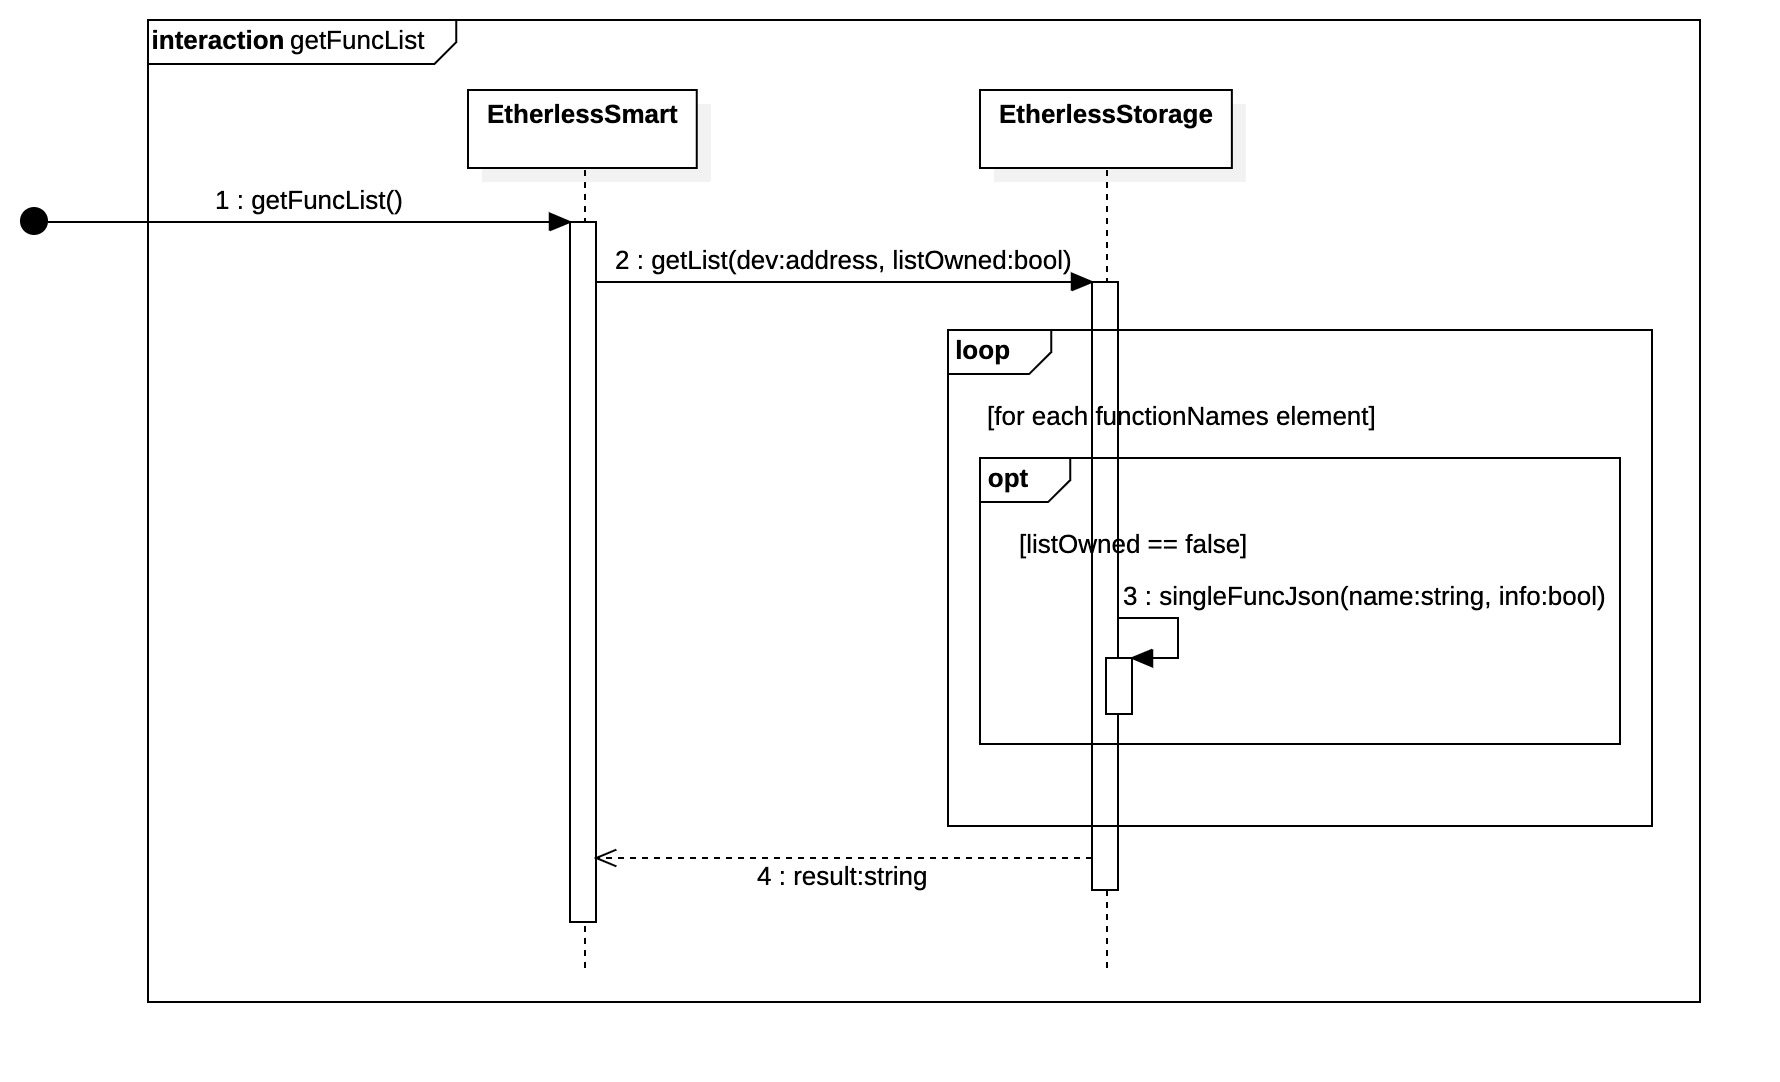
\includegraphics[scale=0.25]{././diagrammi/etherless-smart/sequenza/getFuncList.jpg}}
	\caption{Diagramma di sequenza della richiesta della lista di funzioni}
\end{figure}

\begin{figure}[H]
	\noindent
	\makebox[\textwidth]{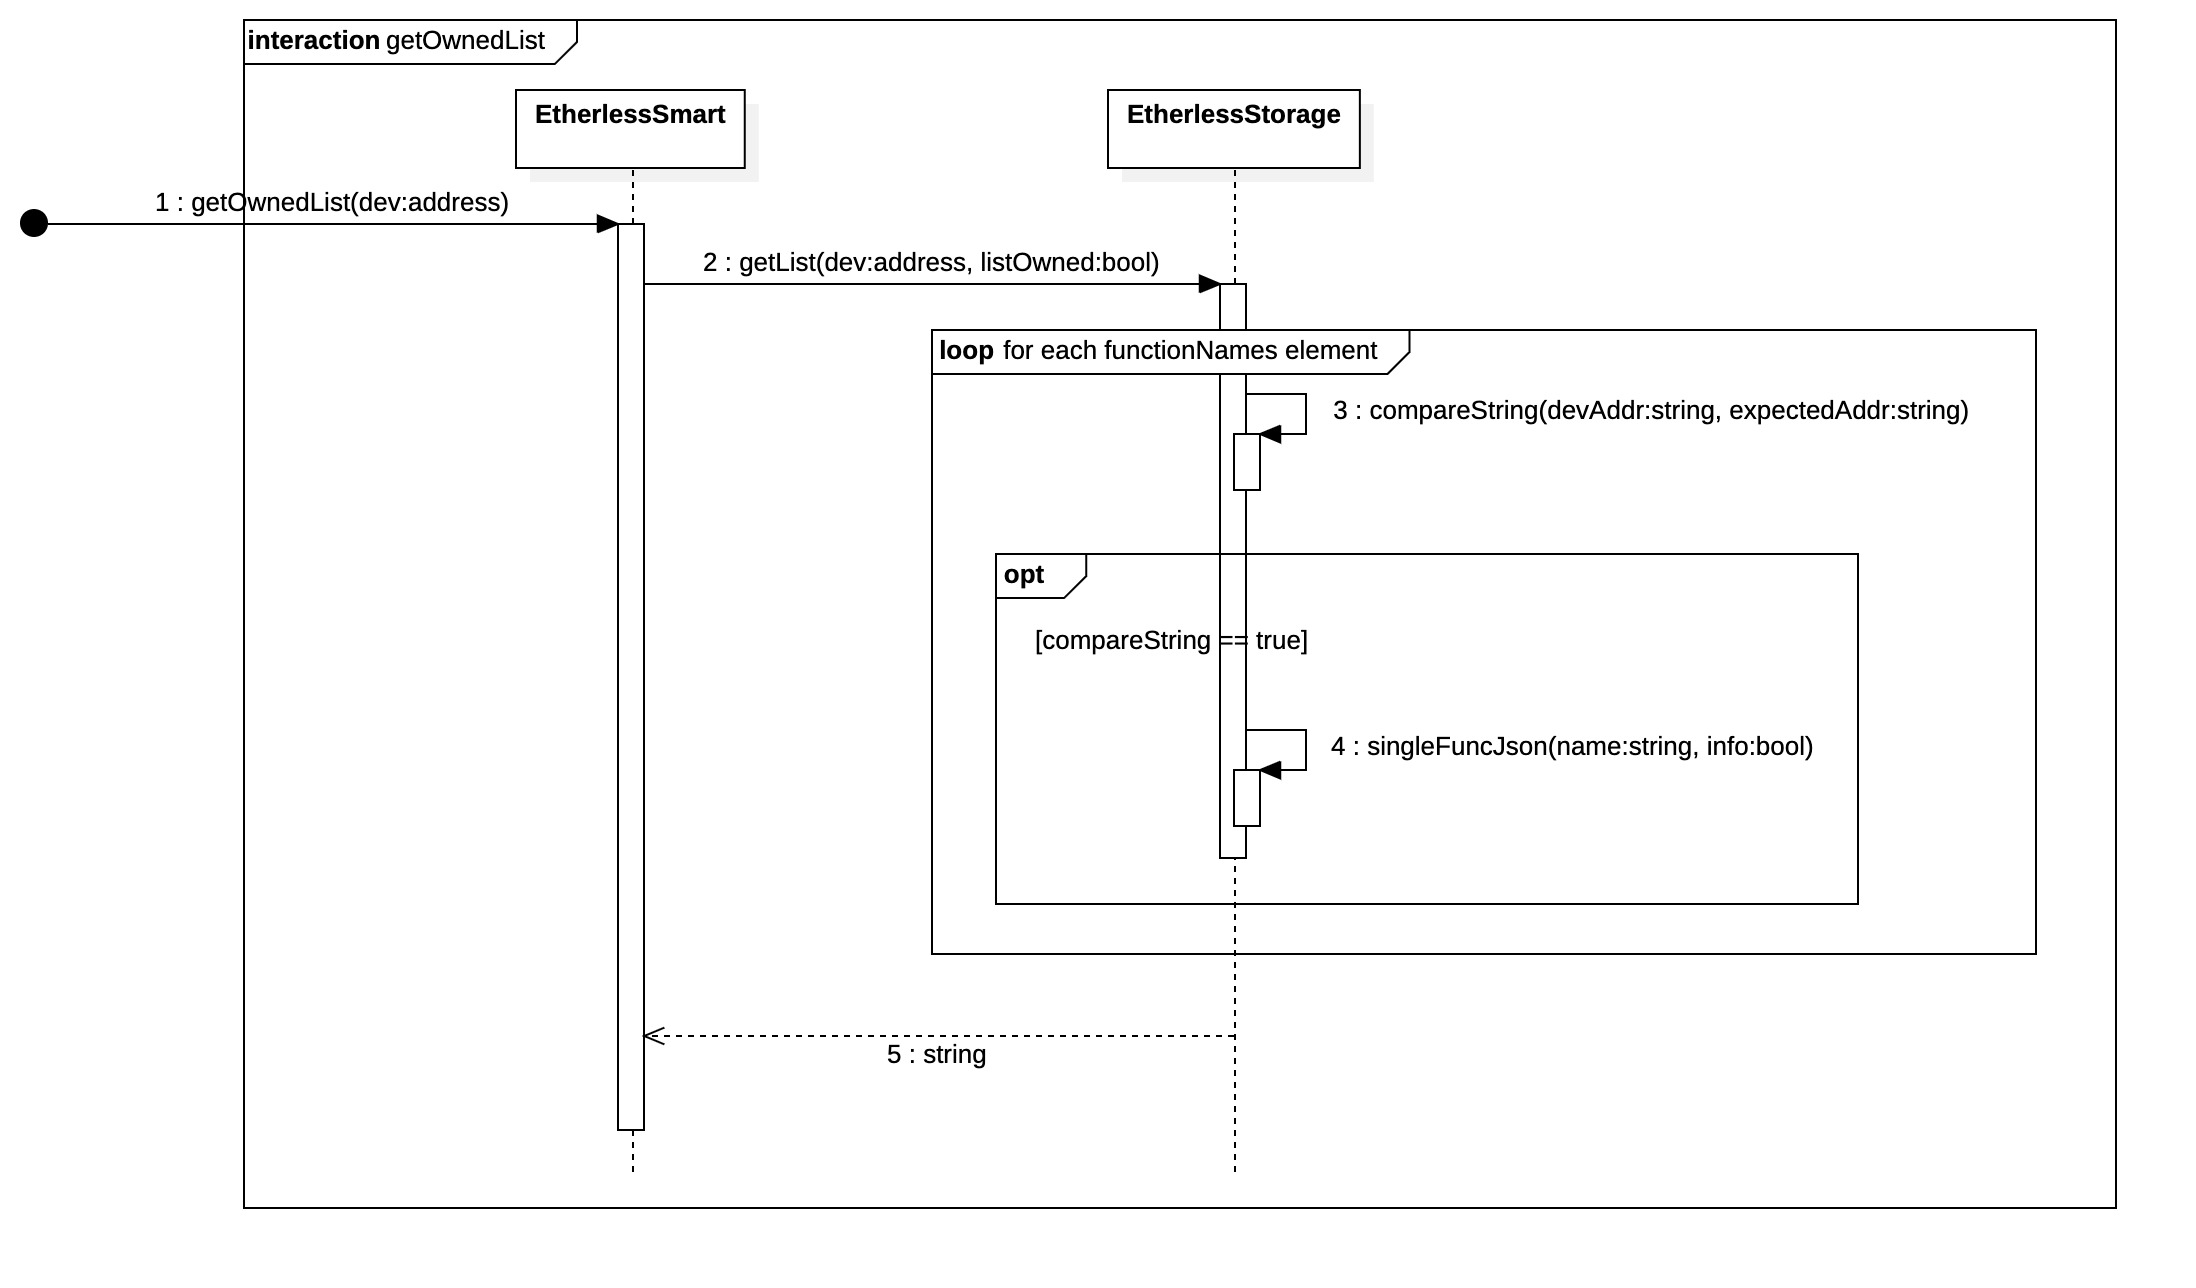
\includegraphics[scale=0.25]{././diagrammi/etherless-smart/sequenza/getOwnedList.jpg}}
	\caption{Diagramma di sequenza della richiesta della lista di funzioni di un dato proprietario}
\end{figure}

\begin{figure}[H]
	\noindent
	\makebox[\textwidth]{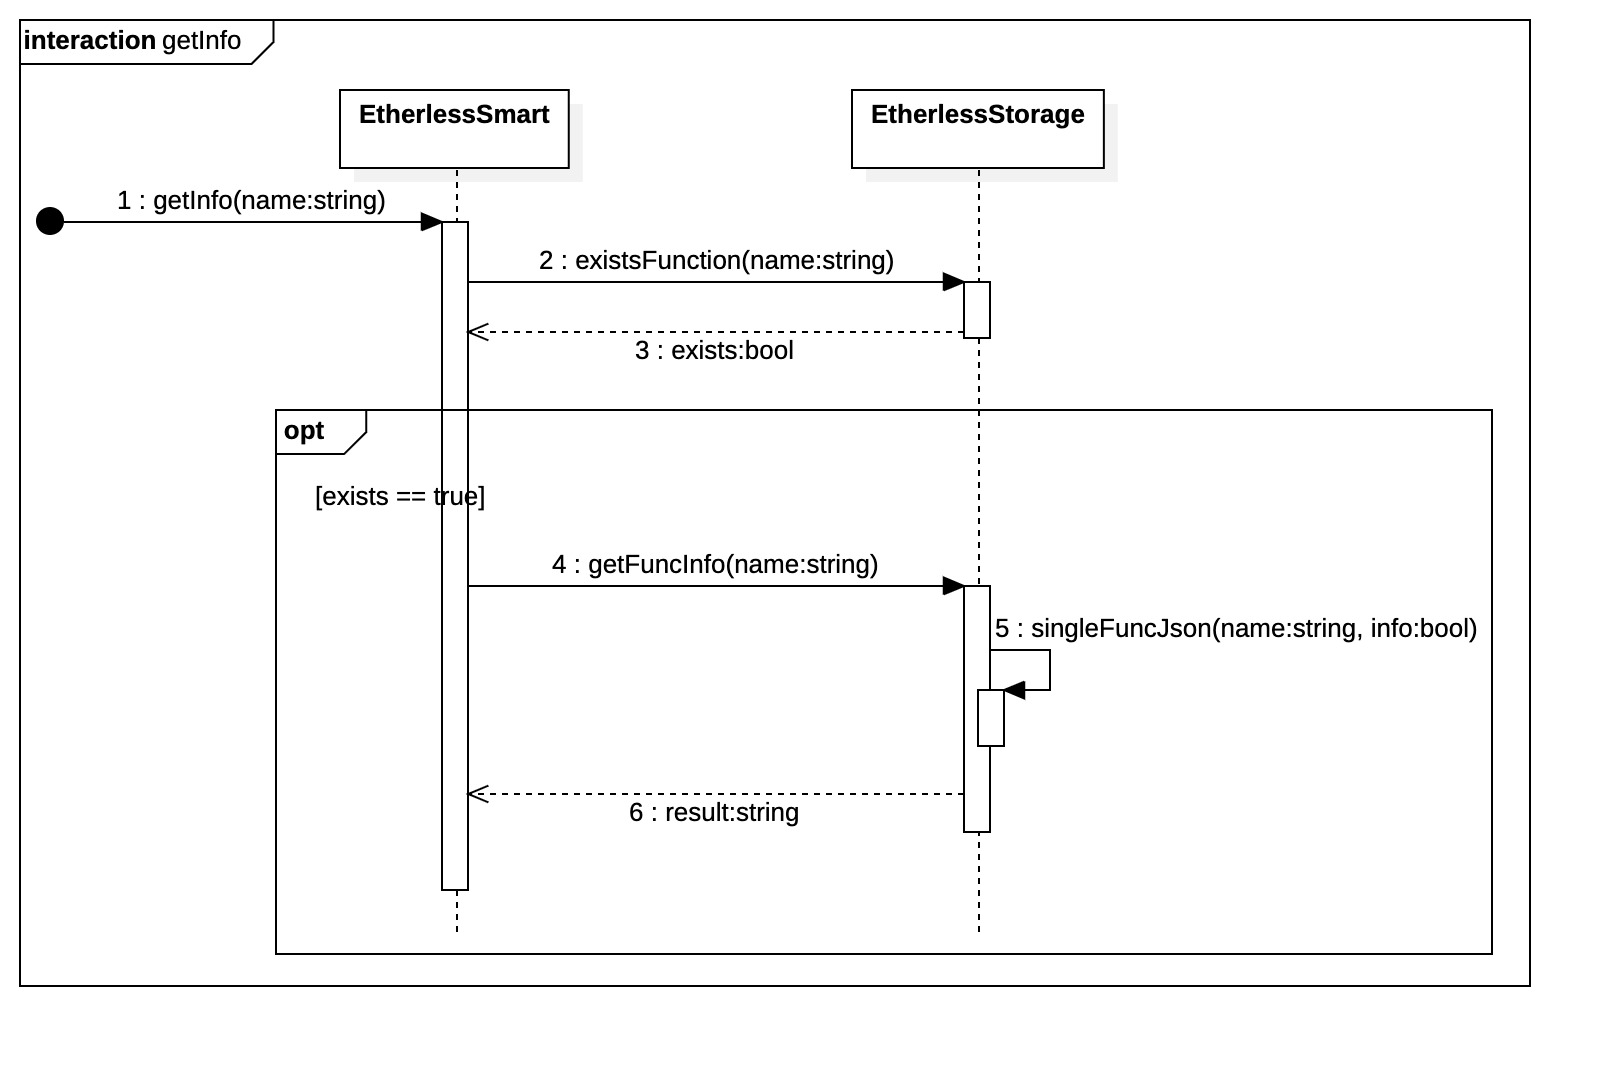
\includegraphics[scale=0.25]{././diagrammi/etherless-smart/sequenza/getInfo.jpg}}
	\caption{Diagramma di sequenza della richiesta delle informazioni dettagliate di una funzione}
\end{figure}

\begin{figure}[H]
	\noindent
	\makebox[\textwidth]{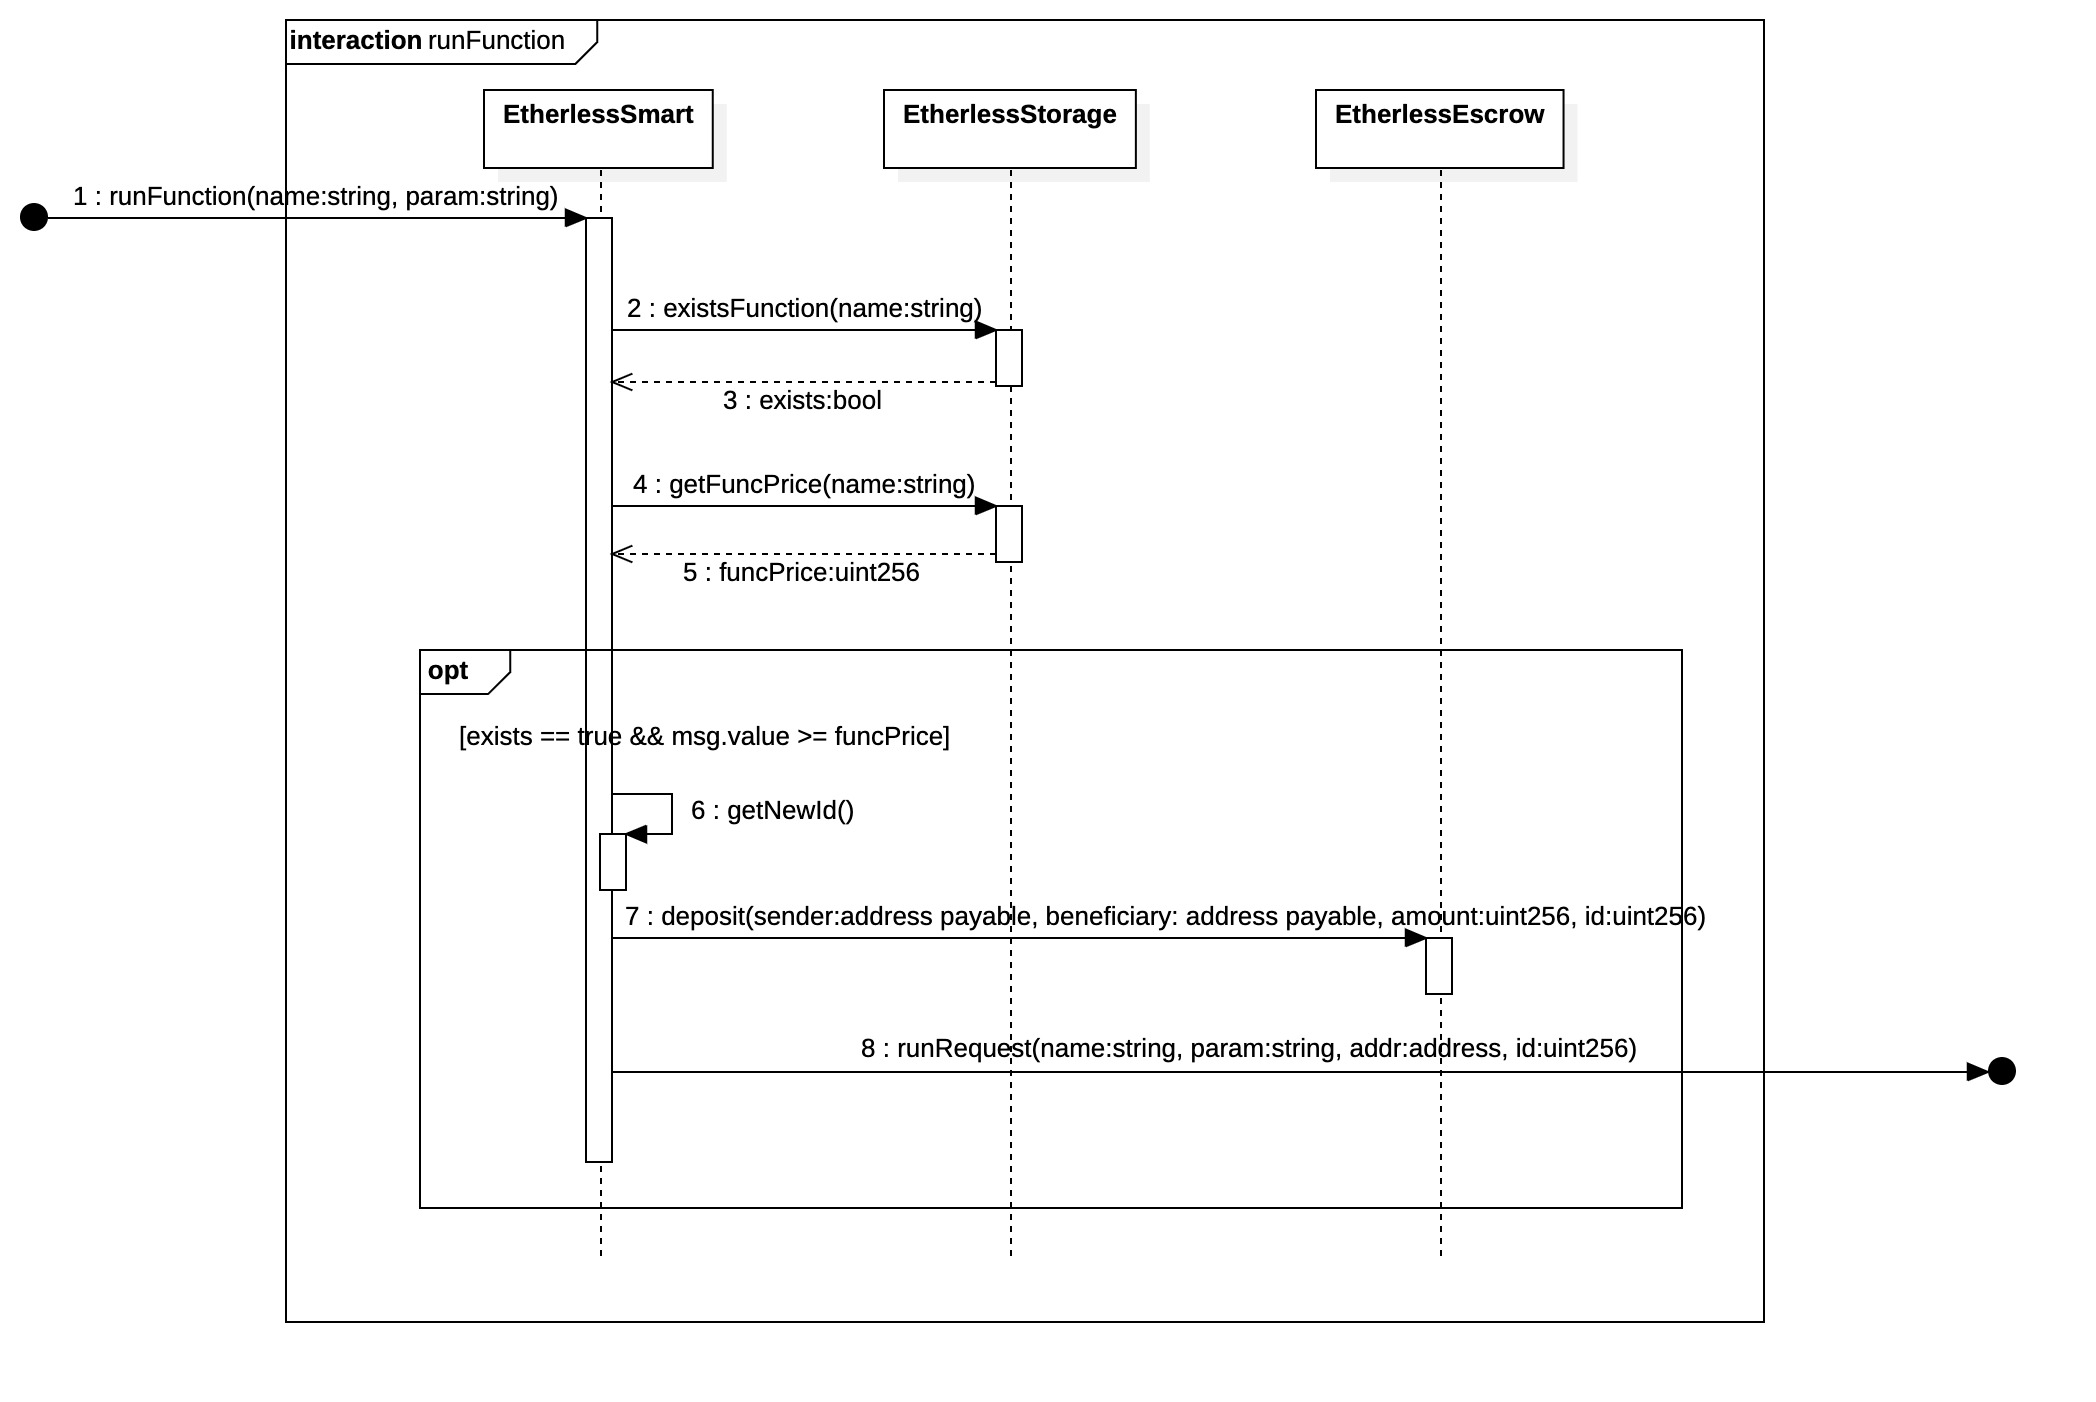
\includegraphics[scale=0.25]{././diagrammi/etherless-smart/sequenza/runFunction.jpg}}
	\caption{Diagramma di sequenza della richiesta di esecuzione di una funzione}
\end{figure}
\begin{figure}[H]
	\noindent
	\makebox[\textwidth]{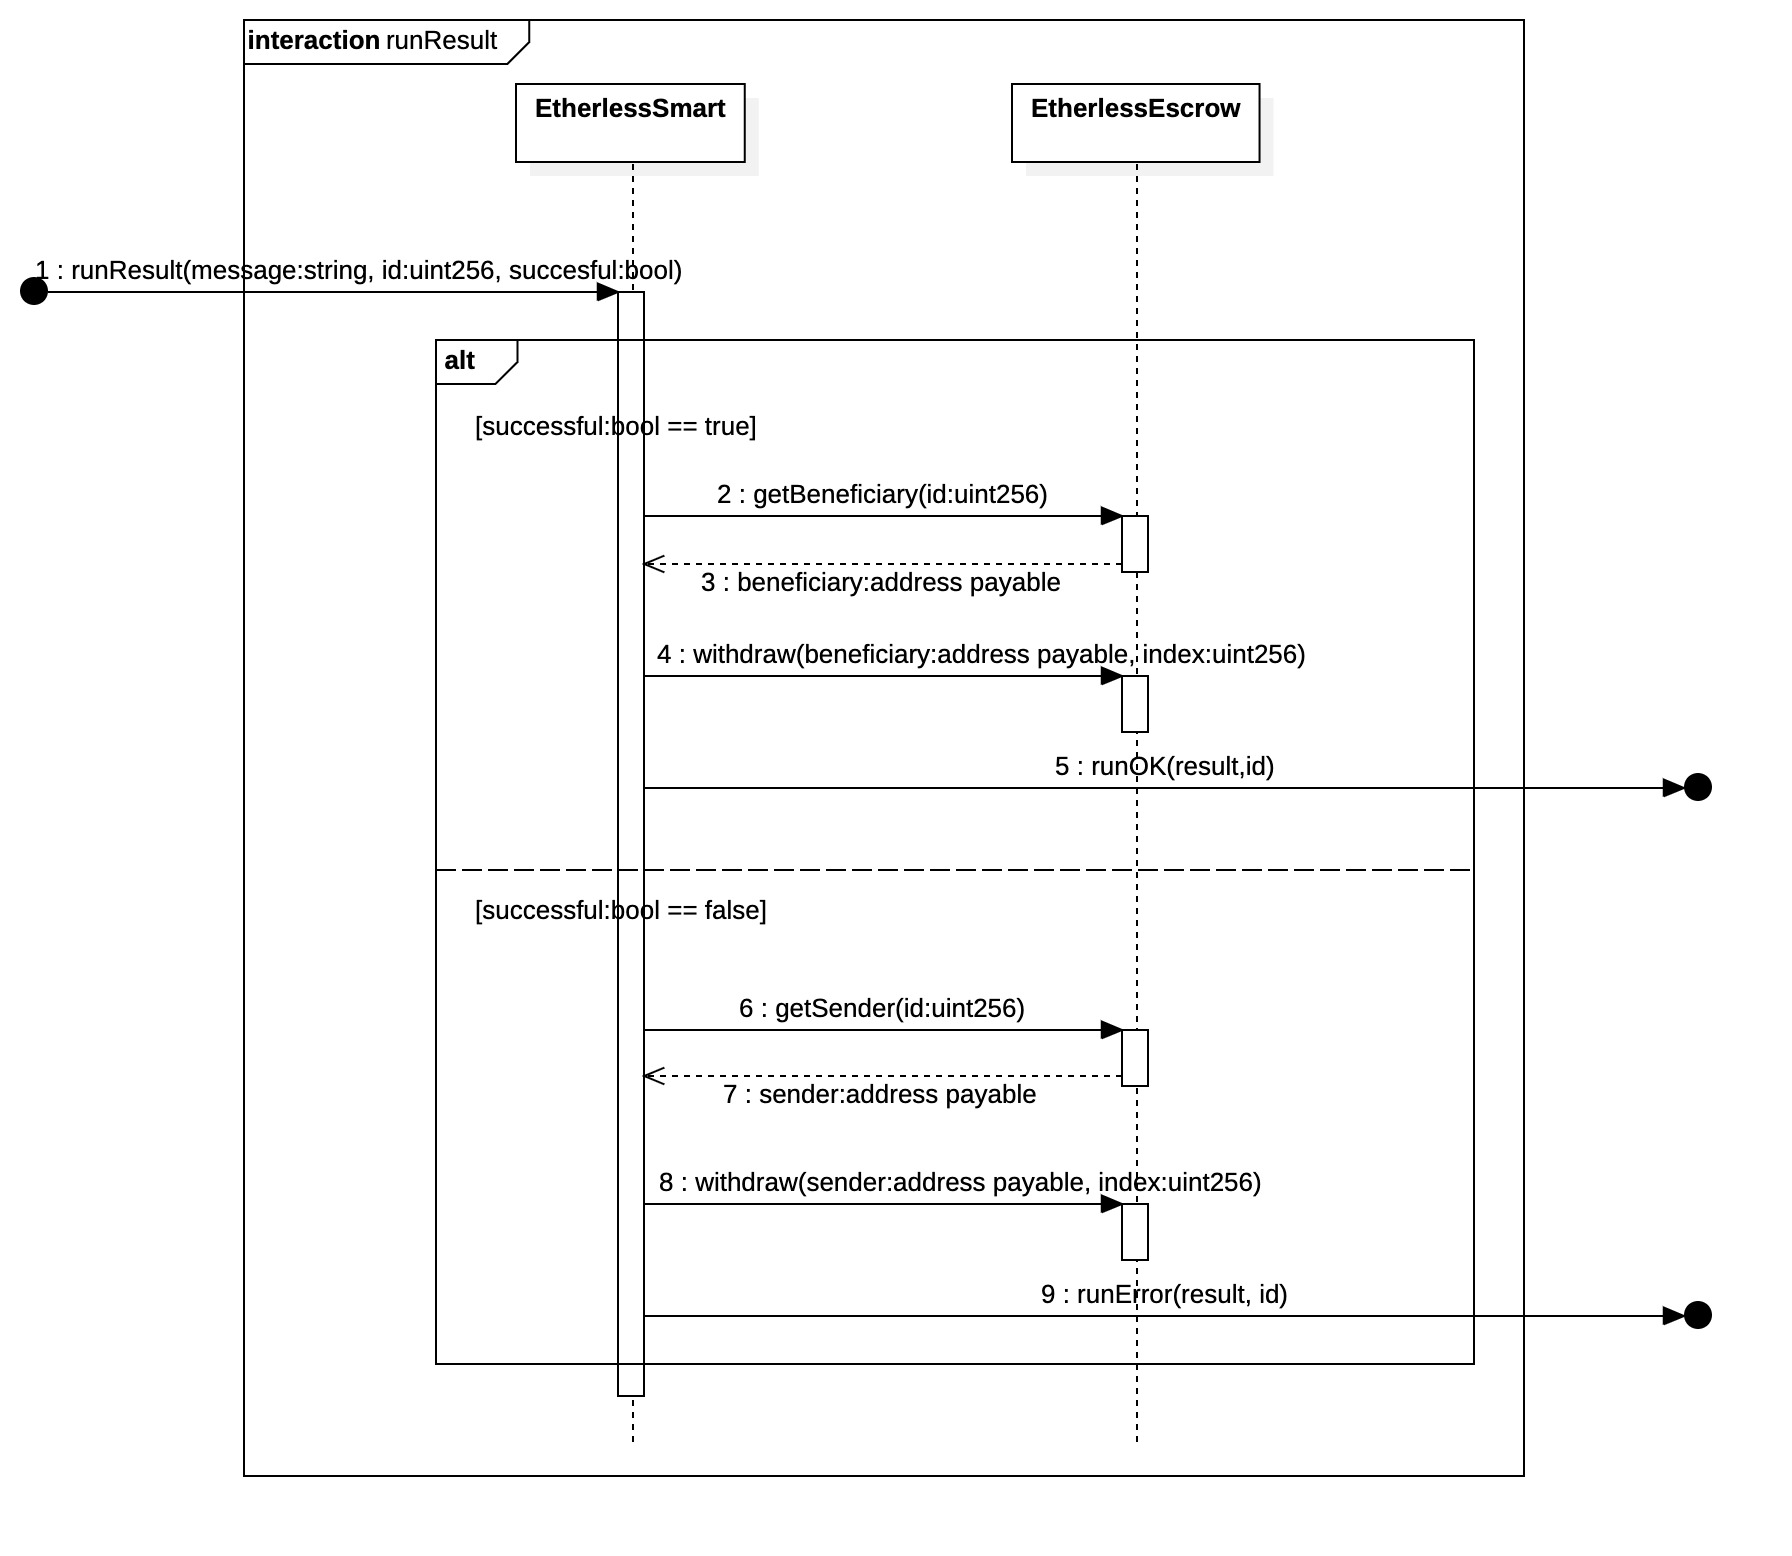
\includegraphics[scale=0.25]{././diagrammi/etherless-smart/sequenza/runResult.jpg}}
	\caption{Diagramma di sequenza della risposta all'esecuzione di una funzione}
\end{figure}

\begin{figure}[H]
	\noindent
	\makebox[\textwidth]{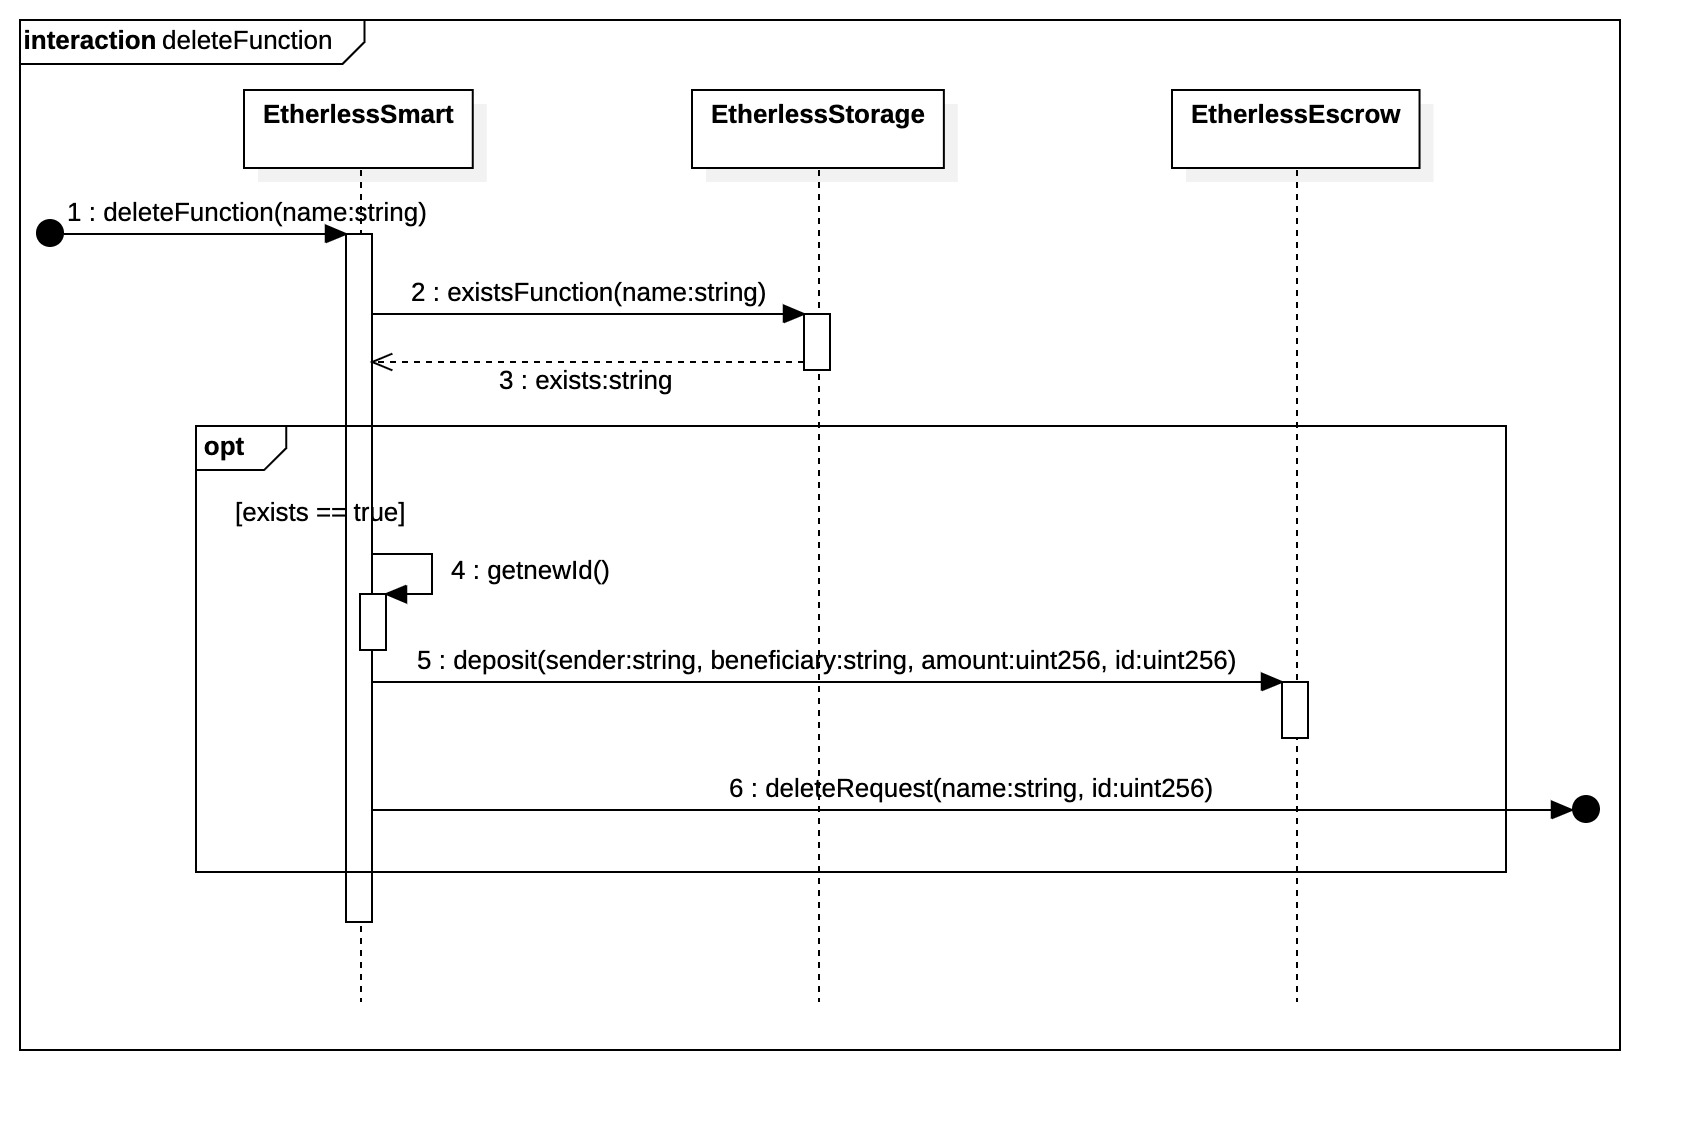
\includegraphics[scale=0.25]{././diagrammi/etherless-smart/sequenza/deleteFunction.jpg}}
	\caption{Diagramma di sequenza della richiesta di eliminazione di una funzione}
\end{figure}
\begin{figure}[H]
	\noindent
	\makebox[\textwidth]{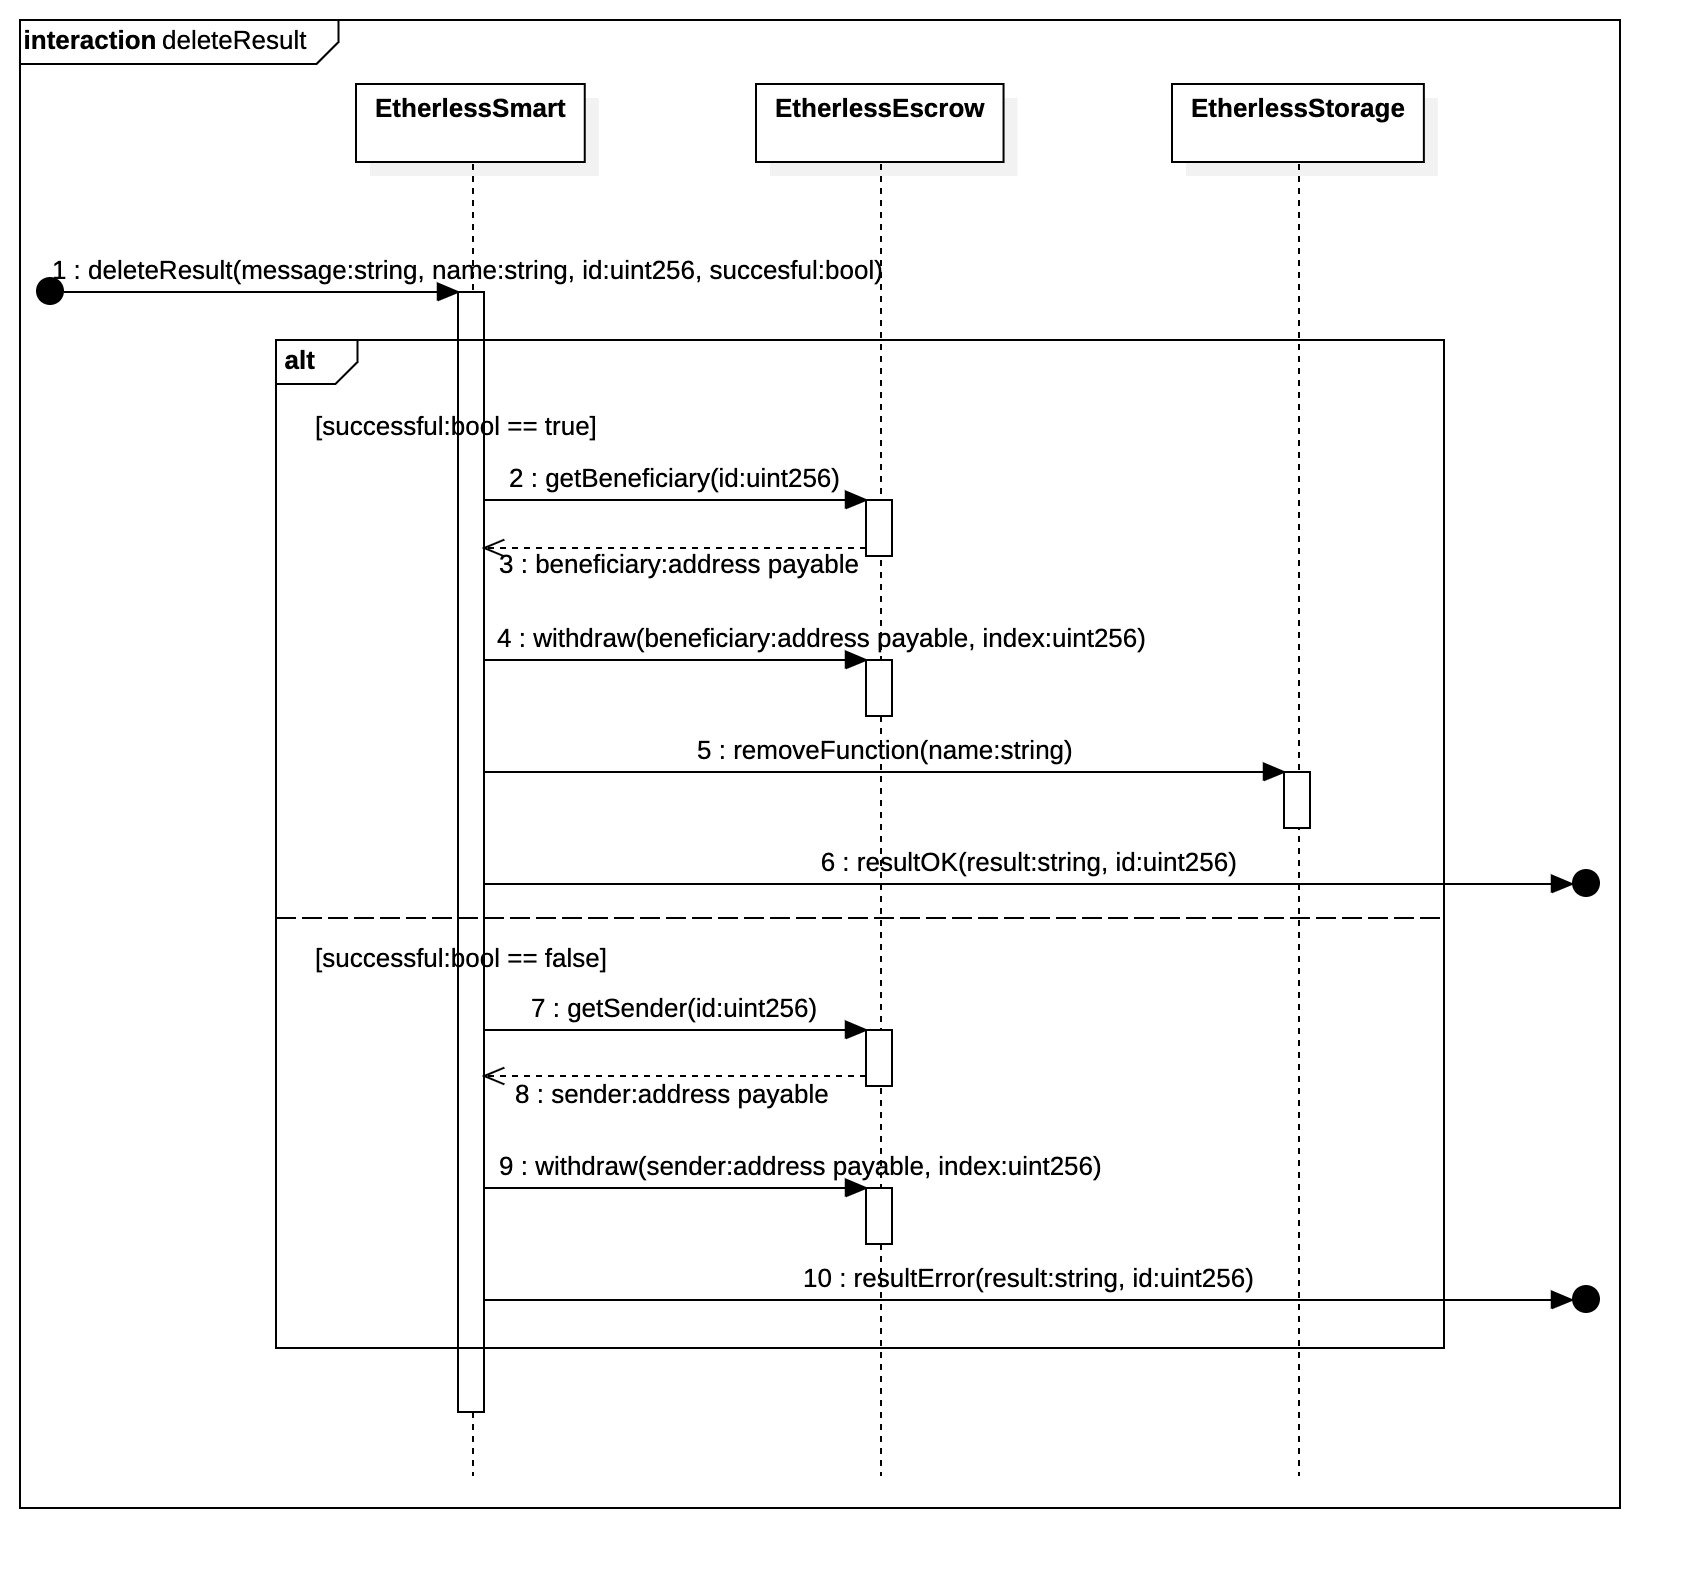
\includegraphics[scale=0.25]{././diagrammi/etherless-smart/sequenza/deleteResult.jpg}}
	\caption{Diagramma di sequenza della risposta all'eliminazione di una funzione}
\end{figure}

\begin{figure}[H]
	\noindent
	\makebox[\textwidth]{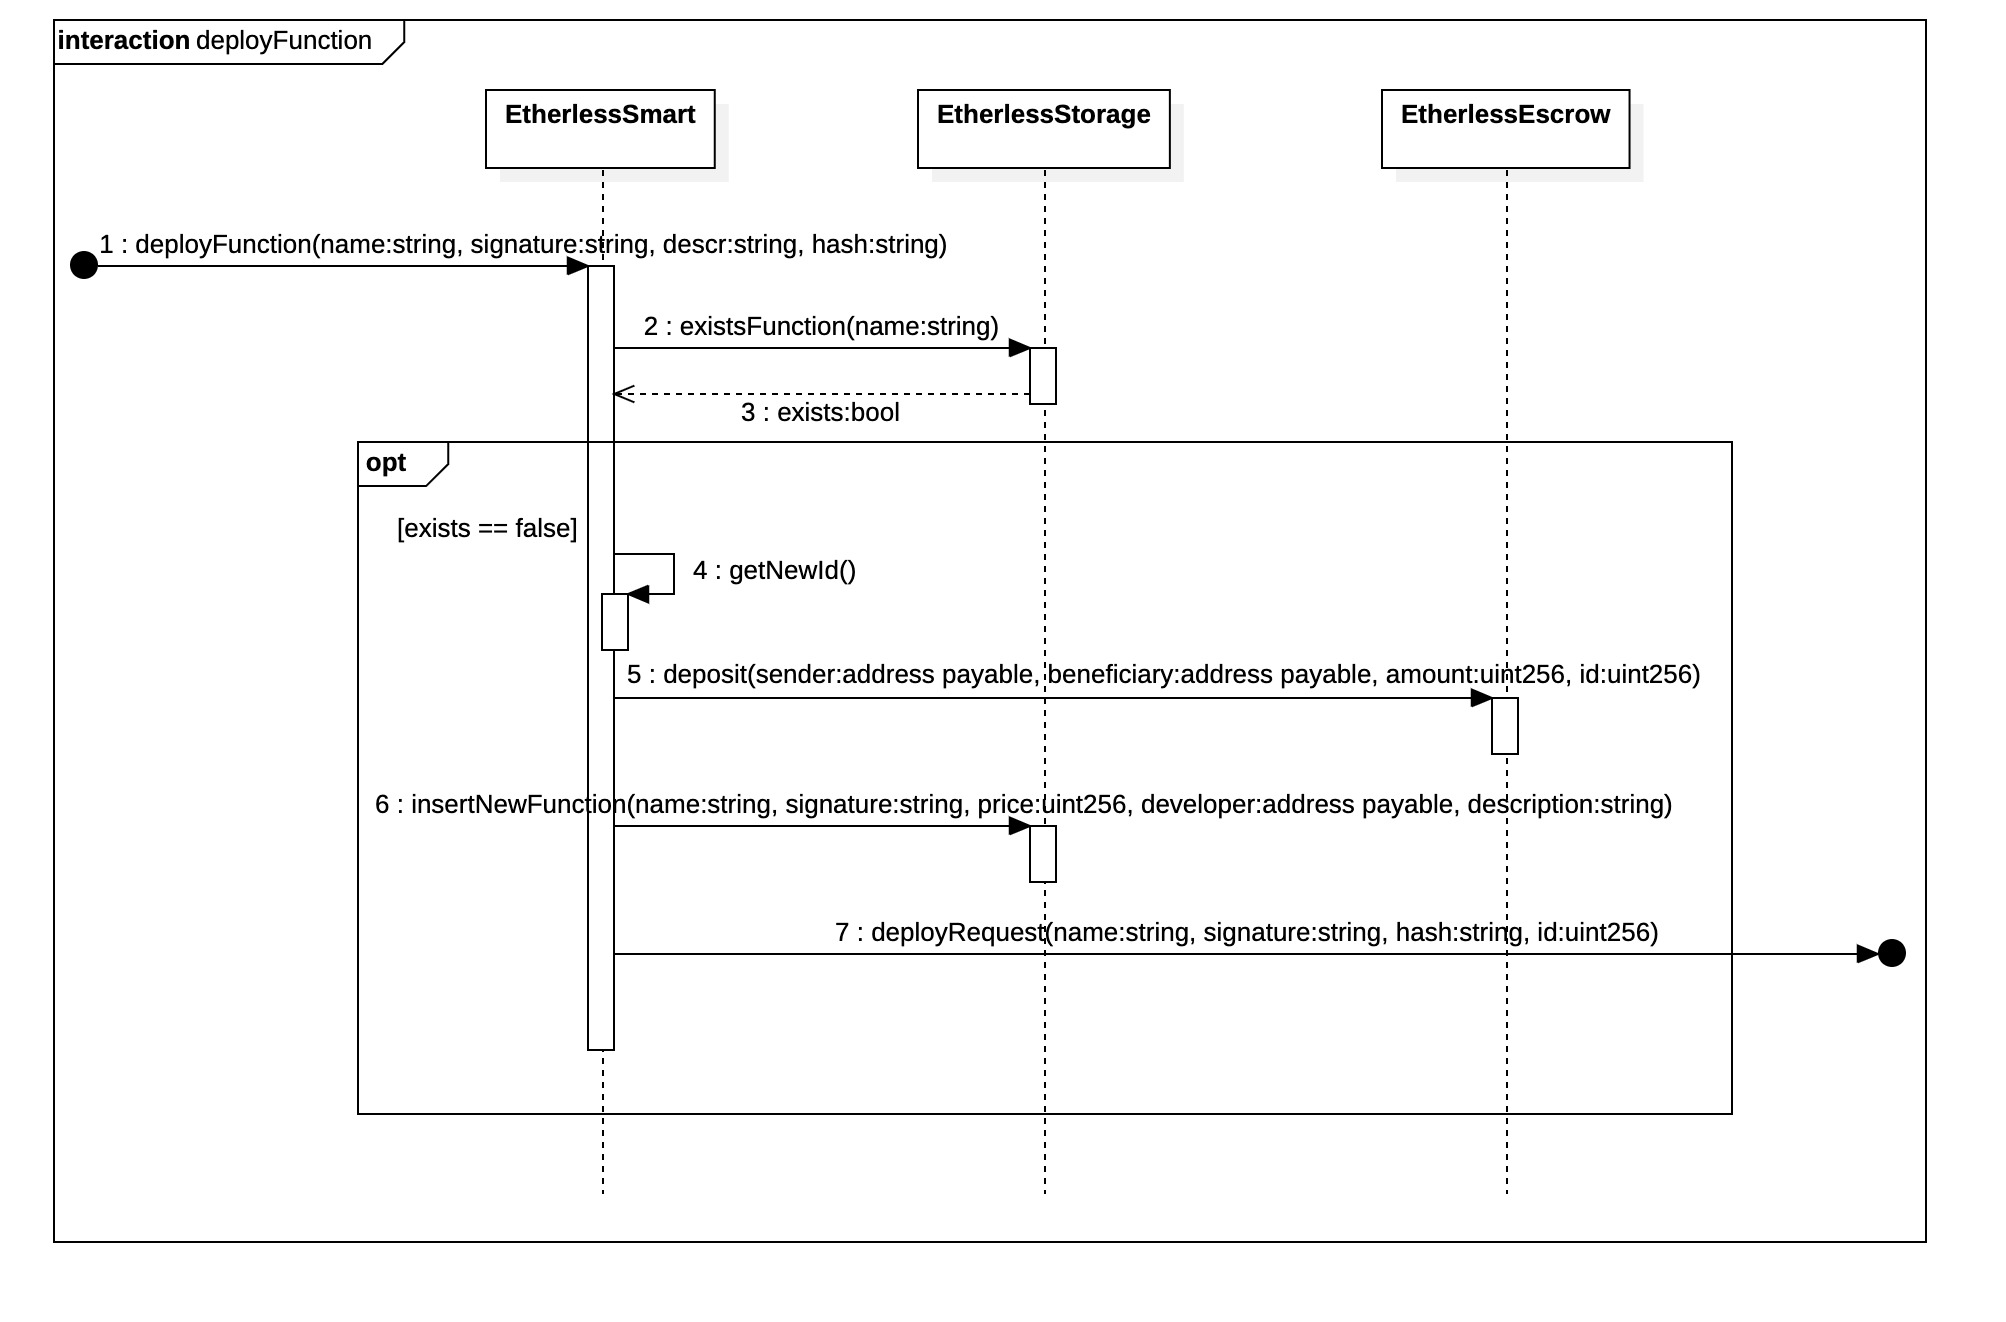
\includegraphics[scale=0.25]{././diagrammi/etherless-smart/sequenza/deployFunction.jpg}}
	\caption{Diagramma di sequenza della richiesta di deploy di una funzione}
\end{figure}
\begin{figure}[H]
	\noindent
	\makebox[\textwidth]{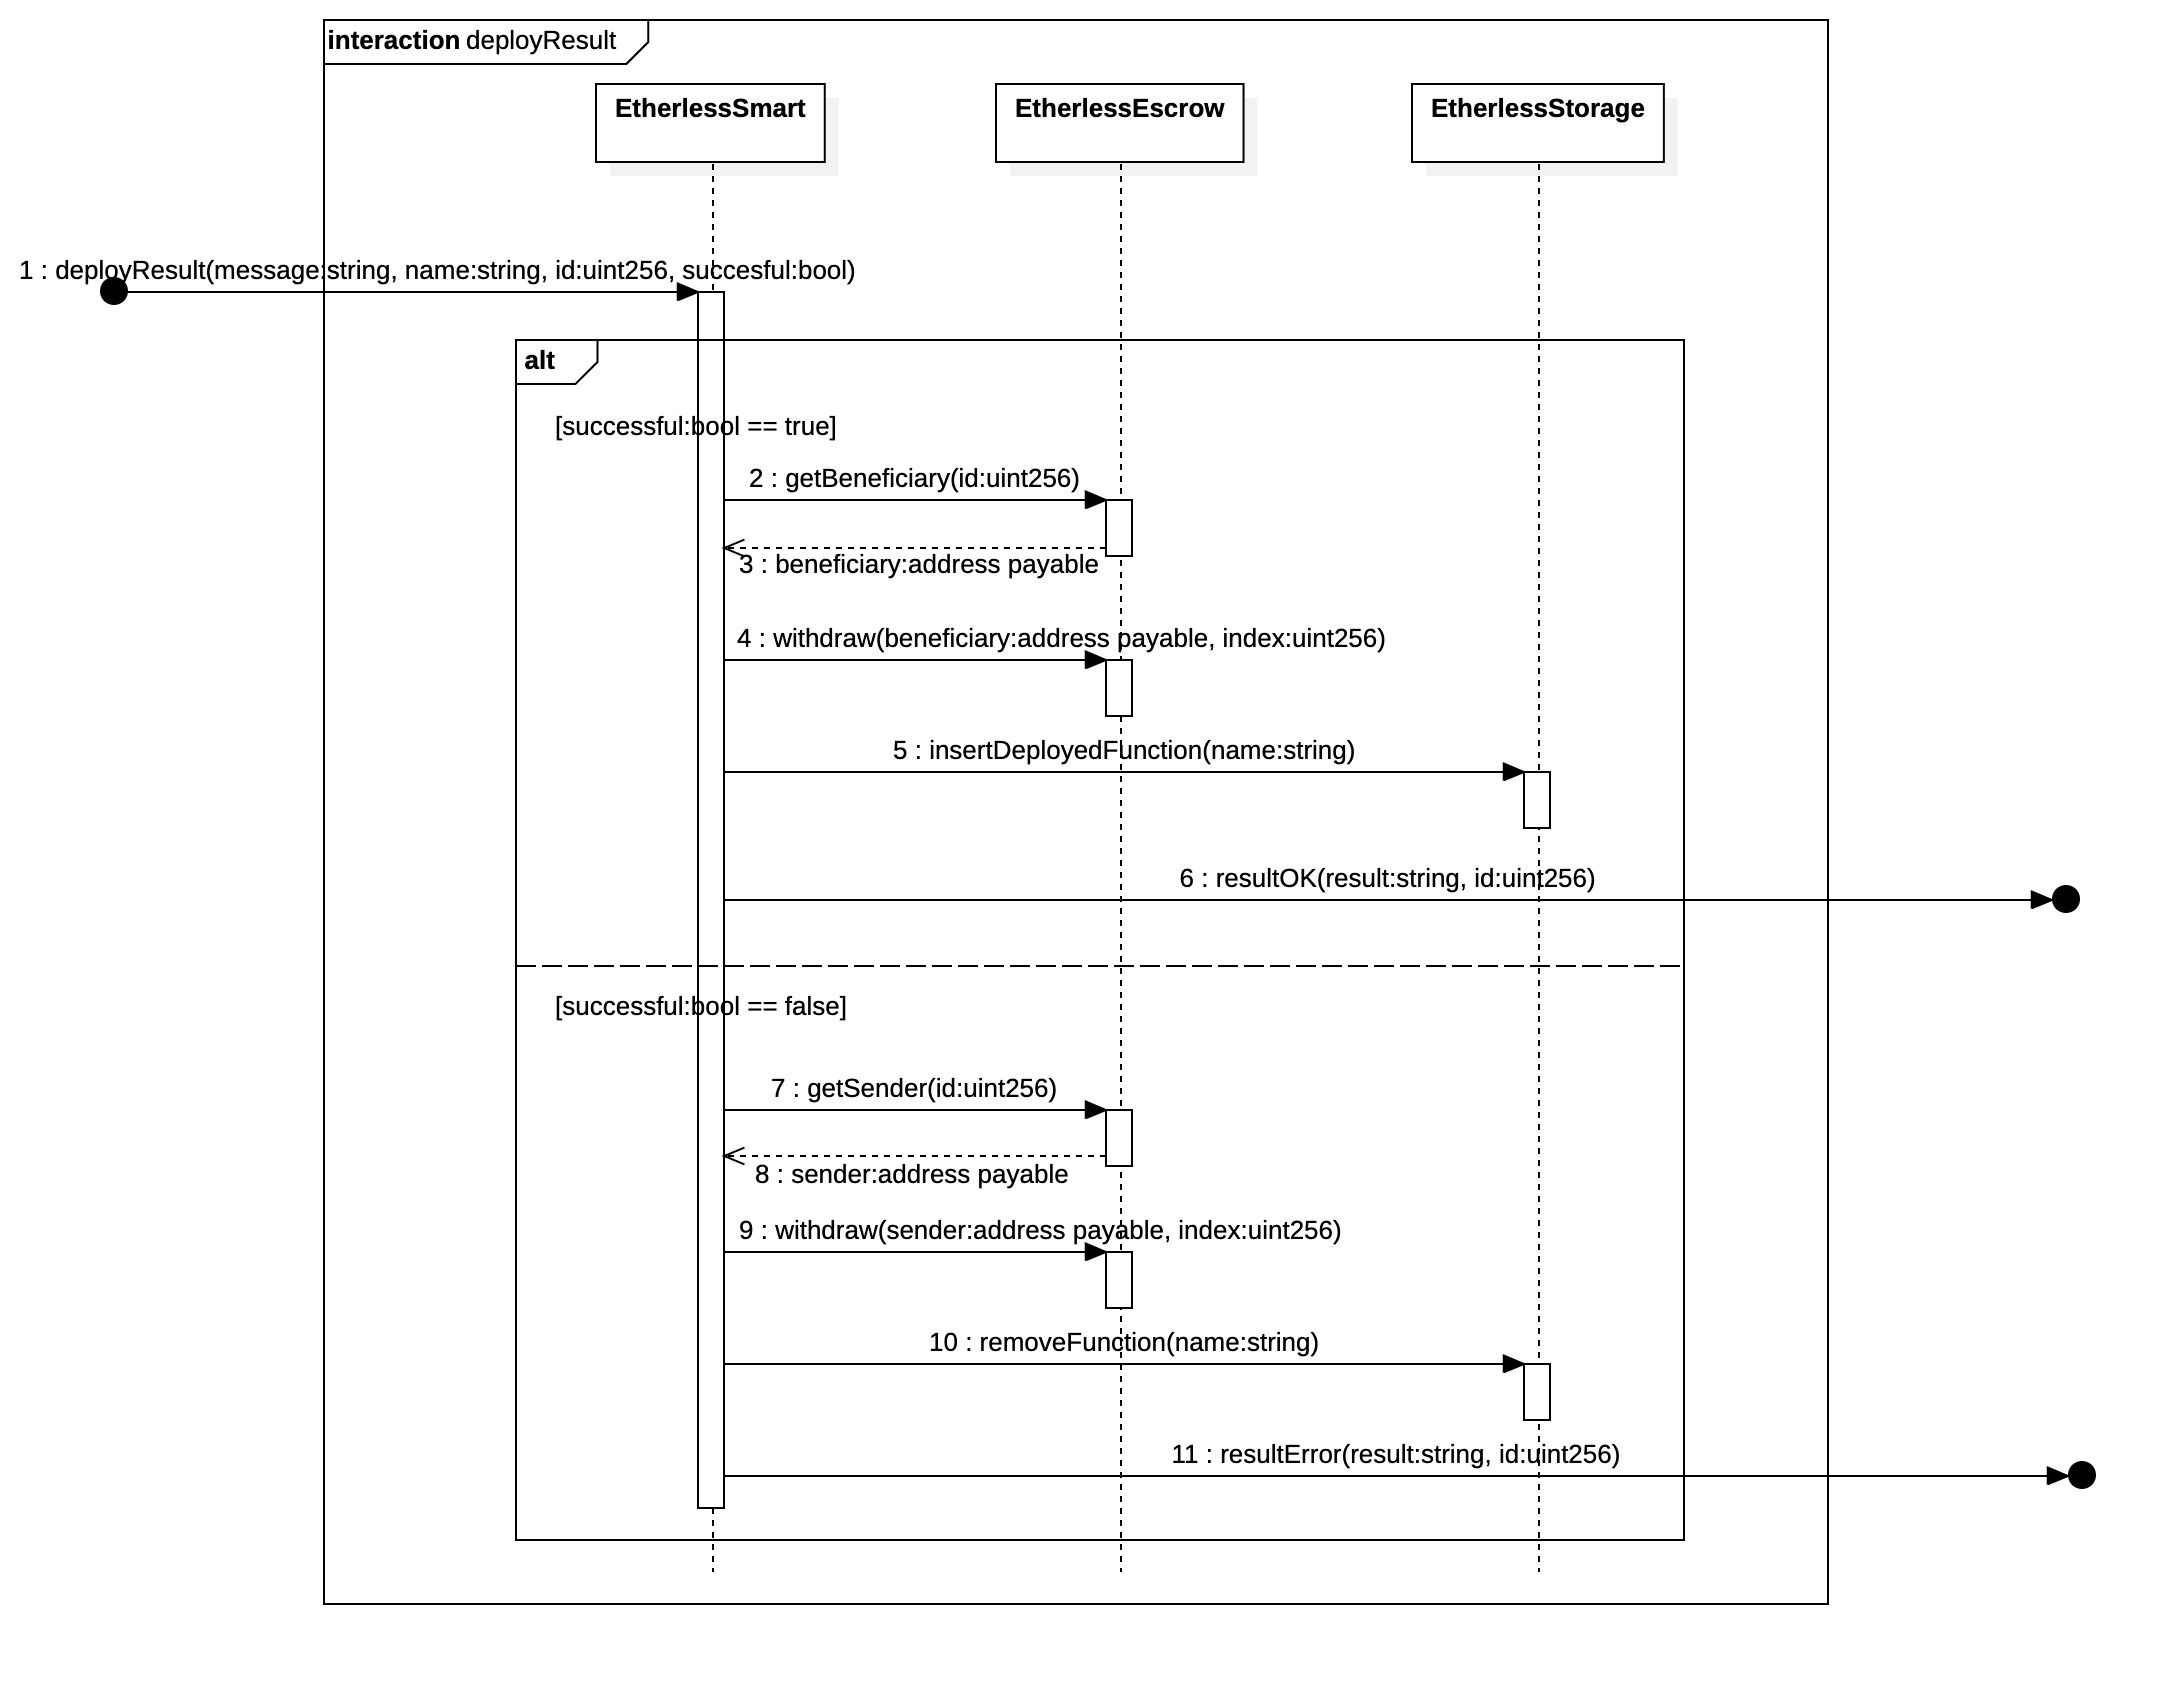
\includegraphics[scale=0.25]{././diagrammi/etherless-smart/sequenza/deployResult.jpg}}
	\caption{Diagramma di sequenza della risposta al deploy di una funzione}
\end{figure}

\begin{figure}[H]
	\noindent
	\makebox[\textwidth]{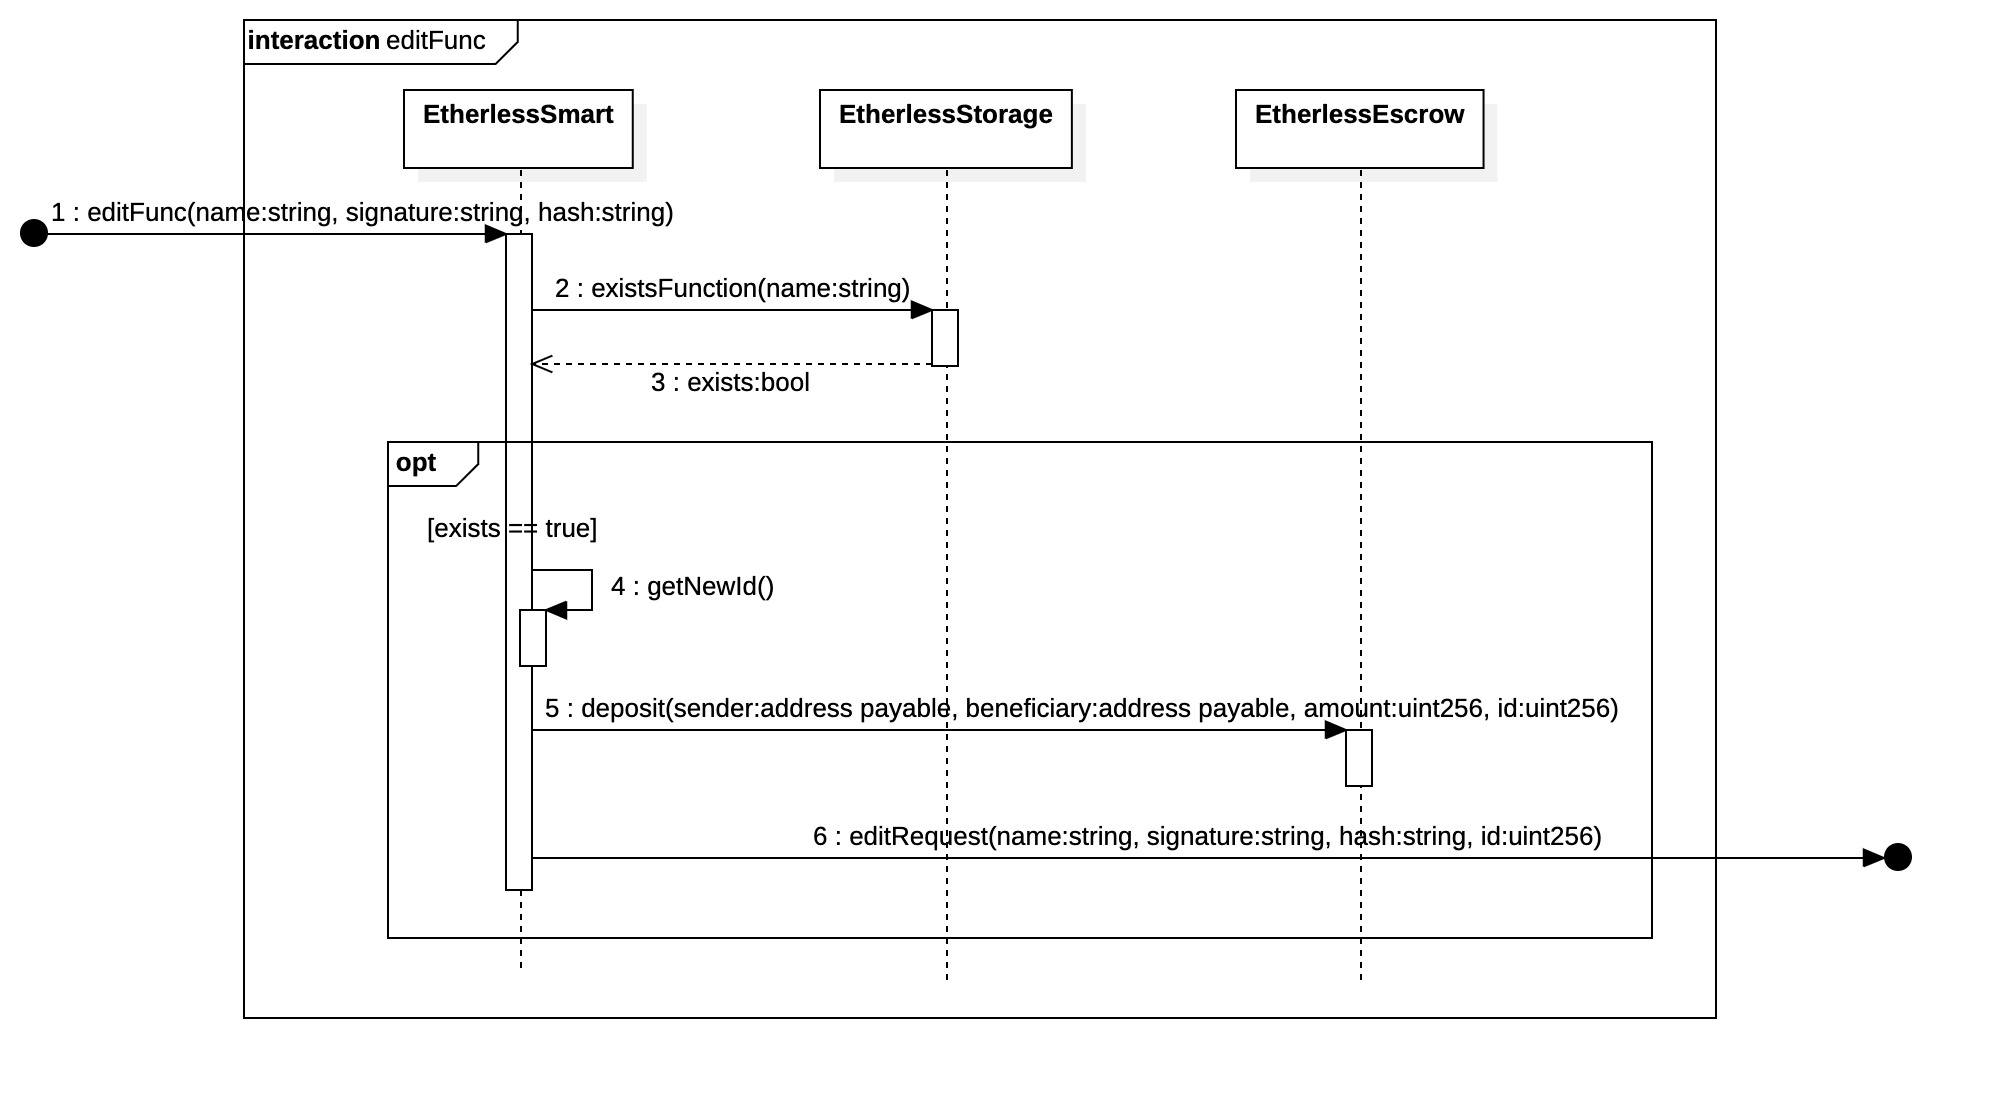
\includegraphics[scale=0.25]{././diagrammi/etherless-smart/sequenza/editFunc.jpg}}
	\caption{Diagramma di sequenza della richiesta di modifica di una funzione}
\end{figure}
\begin{figure}[H]
	\noindent
	\makebox[\textwidth]{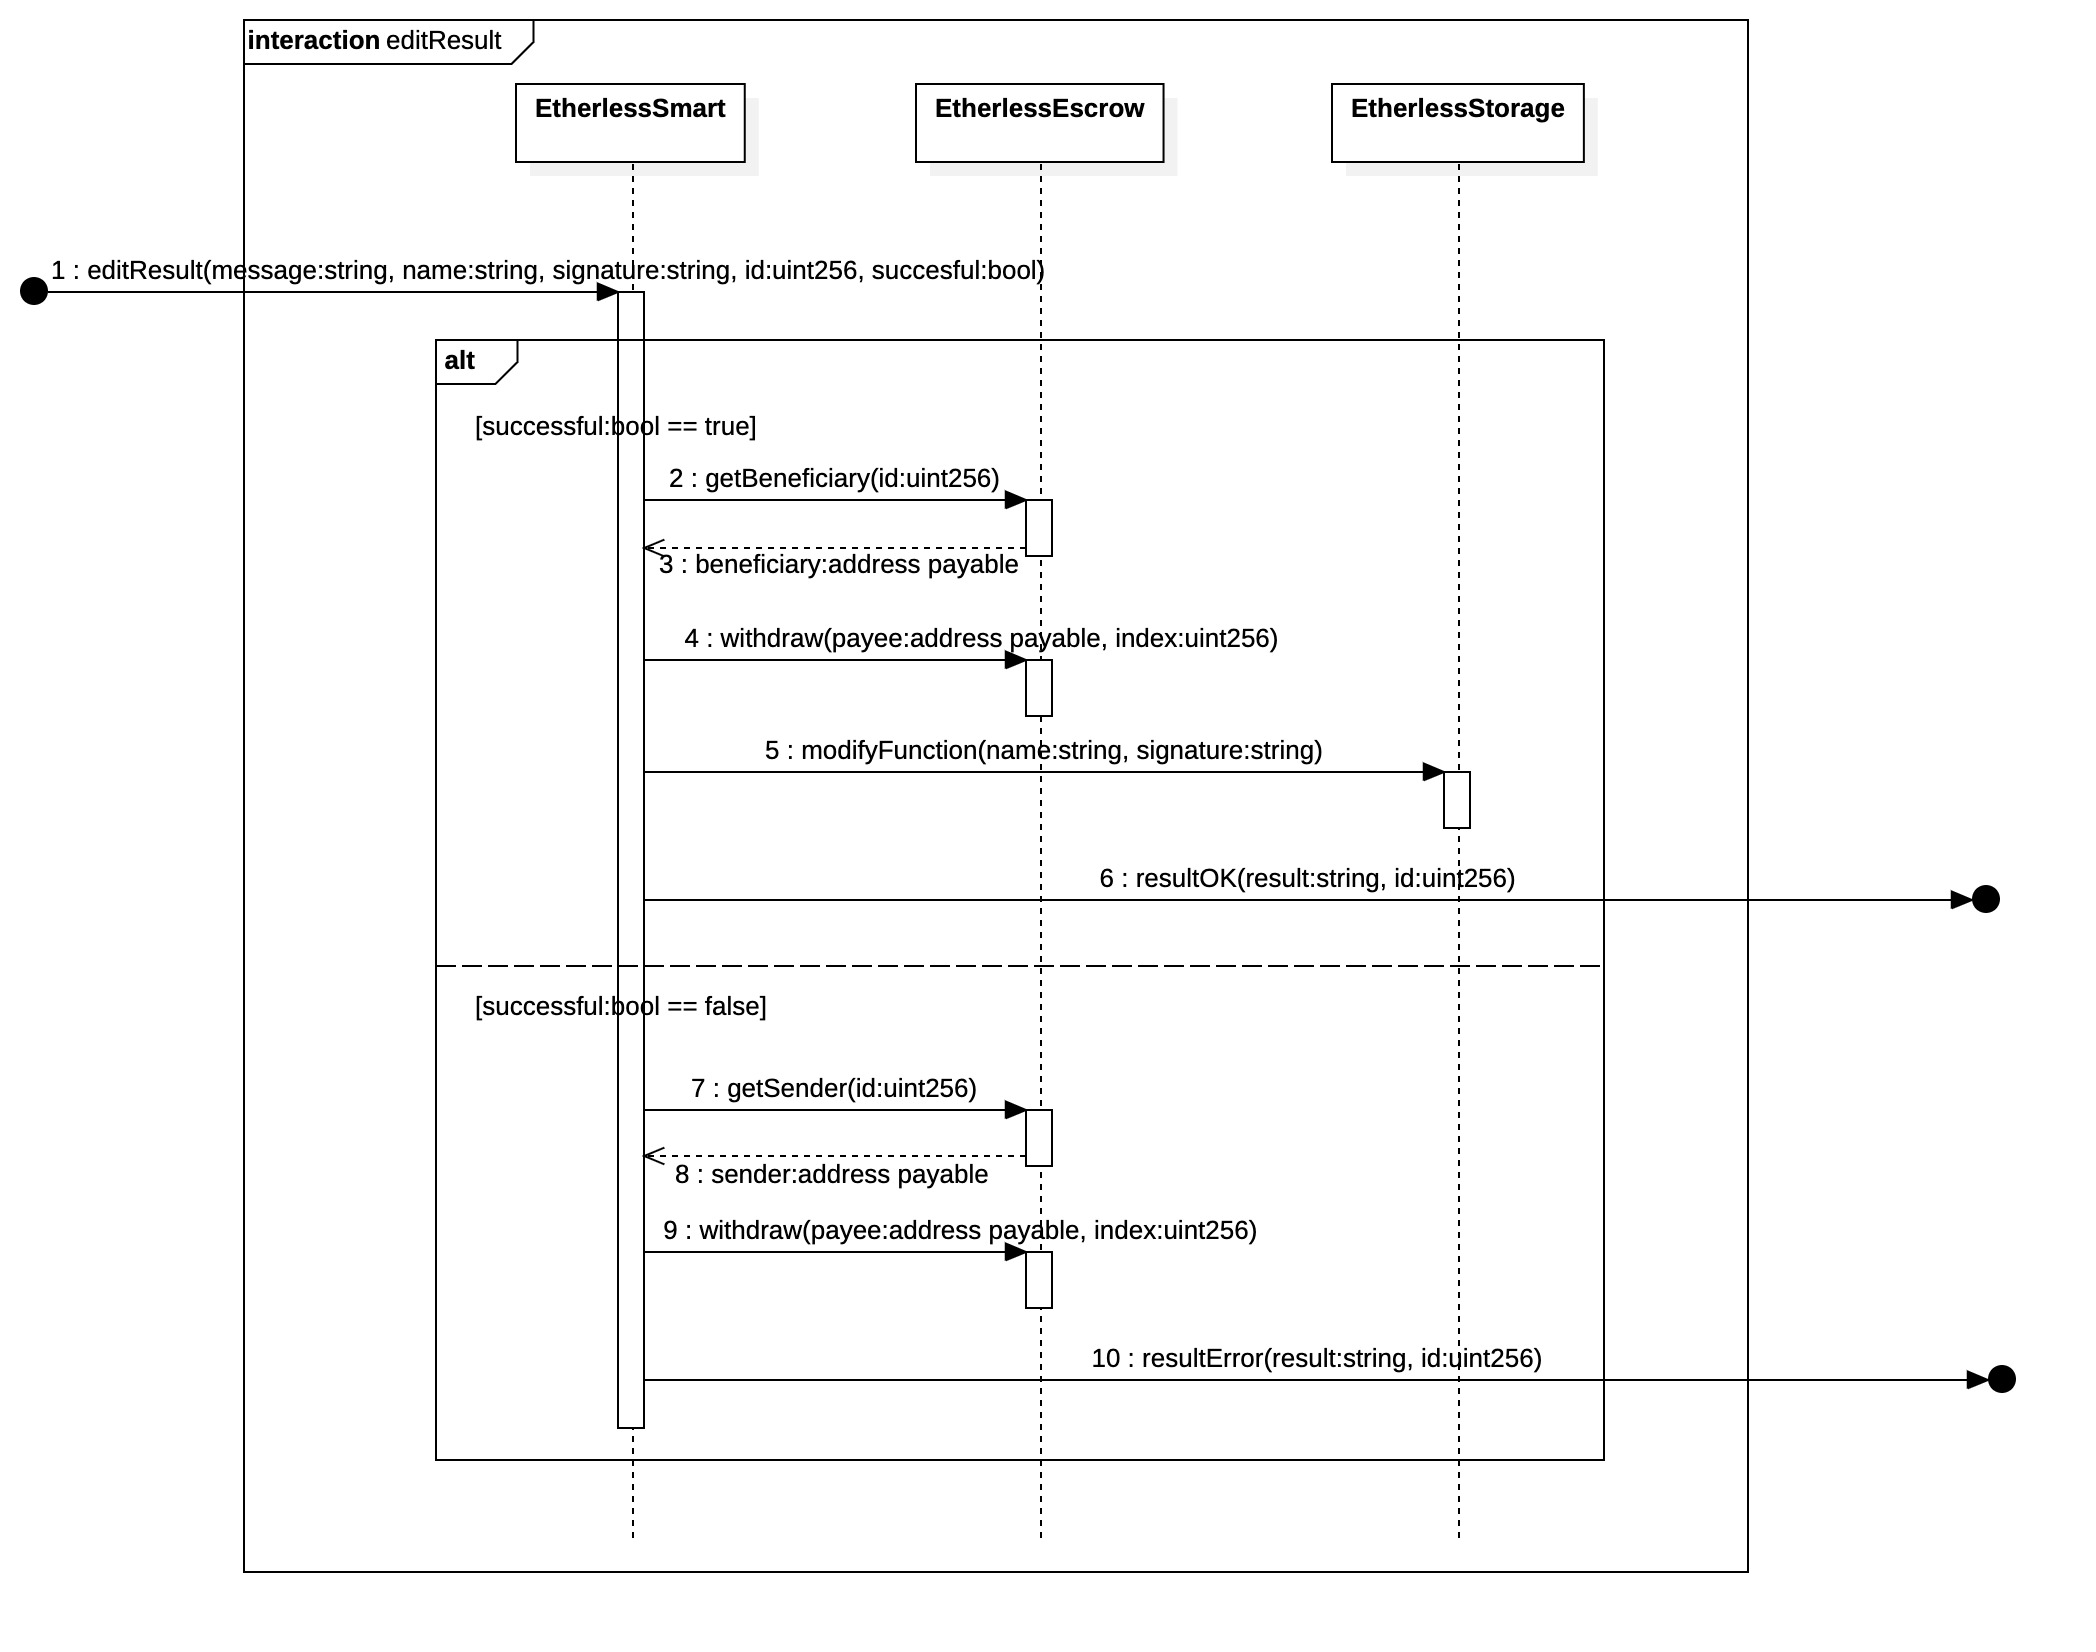
\includegraphics[scale=0.25]{././diagrammi/etherless-smart/sequenza/editResult.jpg}}
	\caption{Diagramma di sequenza della risposta alla modifica di una funzione}
\end{figure}
\newpage
